\documentclass[10pt]{article}

\usepackage{amsmath}
\usepackage{graphicx}
\graphicspath{{images/}}

\begin{document}
\section{Abstract}
In recent times, the increase in the usage of automobiles has caused difficulty in transporting goods between two places.
As a result, the alternative use of employing aerial robots such as drones in transporting goods has gained a lot of popularity
due to the reduced traffic and the effiency and ease of transporting goods from one place to another. 
However, aerial robots face the disadvantage of navigating dynamic obstacles  and being able to interact with the environment in an intelligent 
manner. Due to these difficulties, it is imperative that the drone be equipped with some form amount of intelligence. This paper focuses on how
reinforcement learning can be applied to enable the drone navigate its environment intelligently and efficiently.

\section{Introduction}
Drones in recent times are being used for surveillance in military and for transportation purposes. Amazon currently is trying to commercialize
the use of drones for transporting products from one place to another. The problem of operating a drone is that even if a drone has been 
programmed to follow a specified path using the most intelligent of algorithms, there are bound to be uncertainties. How well the drone responds 
to such situations is of paramount importance as it could mean a drone accidentaly hitting an obstacle, or detecting unreasonable things or
venturing into really dangerous and costly situations.

\begin{figure}[h]
    \centering
    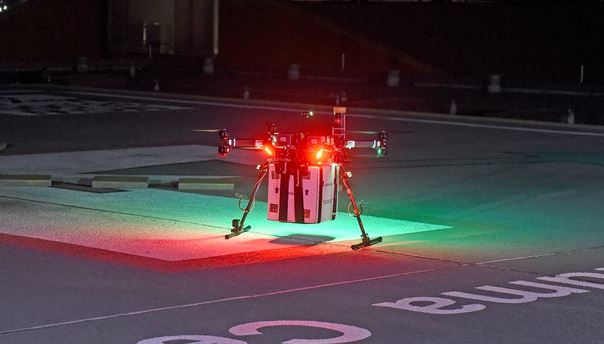
\includegraphics[width=7cm]{kidney}
    \caption{Drone delivering kidney}
    \label{fig:Drone delivering kidney}
\end{figure}
This paper focuses on the first phase of the project which is training a drone to interact with its environment in an intelligent way devoid of 
any sensing capability. Suitable reinforcement learning algorithms are tried and tested to see how well the drone learns- that is, how much reward
can be accumulated from experience. 


\section{Background}
\section{Problem Statement}
\section{Background}
\section{limitations}
\section{Approach}
\subsection{Problem Characteristics}
\begin{itemize} 
  \item \textbf{State Space} -  Continuous State space $\rightarrow$ (Position p,Orientation o)
  \item \textbf{Action Space} - left, right,up,down, forward 
  \item \textbf{Environment} - We focus on \textbf{static environment} for now.
\end{itemize}
\subsection{Qlearning}
Qlearning works with discrete state and action spaces. To apply qlearning to our problem, we discretize the continous state space 
and work from there. 

\begin{equation}
  Q(S_t,A_t) \leftarrow Q(S_t,A_t) + \alpha[R_{t+1}+\gamma \max\limits_a Q(S_{t+1},a)- Q(S_t,A_t)]
\end{equation}

\subsection{Results}
\subsection{Deep Qlearning}
\subsubsection{Problems with Qlearning}
\textbf{Qlearning} is not an appropriate solution as:
\begin{itemize}
  \item \textbf{State space is huge(continuous state space)}- The drone can be in particular position with some orientation. 
  \item \textbf{Slow to learn} - Qlearning tries to learn the value of each state space. This is not ideal as state space
        close(suitable metric) together coudld have yield similar values. Therefore, a method which approximates the value function
        using a suitable function is more desirable.
  \item \textbf{Huge memory} - Qlearning learning requires a lot of memory space for this problem
\end{itemize}
\subsubsection{Function Approximation}
This section contains mater from David Silver slides. Refer to David silver or sutton Button for in depth explanation. \\ \\

The goal then is to find parameters w, that minimizes the distance(suitable metric) between the actual value function $v_\pi(s)$ and 
the approximate value function $\bar{v}(s,w)$.
The cost function then becomes,
\begin{equation}
    J(w) =  E_\pi[(v_\pi(S) - \bar{v}(S,w))^2]
\end{equation}


\subsection{Results}
\section{Implementation}
\section{Analysis}
\section{Conclusions}
\section{Future Work}
\section{Bibliography}
\end{document}



